%!TEX root = ../dissertation.tex

\chapter{Implémentation}
\label{chp:impl}

%Example of \autoref{tab:1}, made using %\url{https://www.tablesgenerator.com/}.


%\begin{table}
%    \centering
%    \begin{tabular}{@{}ll@{}}
%        \toprule
%        \textbf{A} & \textbf{B} \\ \midrule
%        1          & 2          \\
%        3          & 4          \\ \bottomrule
%    \end{tabular}
%    \caption{Interesting results.}
%    \label{tab:1}
%\end{table}

\section{Tuteur}
Dans les STIs, le tuteur joue un rôle très important. Il supervise, oriente et évalue l'apprenant tout au long du processus d'apprentissage. C'est la composante des STI qui implémente l'adaptabilité du système en
offrant la possibilité d'encadrer chaque apprenant de manière personnalisée à travers des interactions soigneusement élaborées.

Dans notre système, les interactions entre le tuteur et l'apprenant se font selon une approche de \textbf{Coaching}, qui est une méthode d'enseignement dans laquelle le tuteur et l'apprenant collaborent à la construction de solutions \cite{vanlehn1996conceptual}. Dans cette méthode l'interaction apprenant-tuteur s'ajuste en fonction des progrès de l'apprenant. 

Pour être capable de remplir efficacement ses fonctions, le comportement de notre tuteur se base sur des règles tutorielles. Par exemple:
\begin{itemize}
    \item Si l'apprenant pose une question pas appropriée, alors l'interpeller et lui rappeler (donner une piste) les types de questions à poser dépendant du contexte.
    \item Si l'examen demandé par l'apprenant ne cadre pas avec le contexte, alors l'interpeller et l'orienter si nécessaire.
    \item Si le différentiel proposé par l'apprenant est trop éparse et divergeant, alors l'interpeller et l'orienter si nécessaire.
\end{itemize}


Pour implémenter ces règles nous proposons l'outil \textbf{JESS} (Java Expert System Shell) qui est une API entièrement développée en Java pour la création des systèmes experts à base de règles.

\section{Interface Utilisateur : prototypage}

La conception de notre interface utilisateur étant basée sur la conception centrée sur l'utilisateur, nous présentations dans cette partie la dernière phase de celle ci: L'implémentation.

Nous avons utilisé l'approche Hi-Fi ( High Fidelity) pour le prototypage de nos interfaces utilisateur. Il s'agit d'une représentation avec un maximum de détails.
\subsection{Outils Utilisés pour le prototypage}
\subsubsection{Pour le prototypage}
Notre choix s'est porté sur l'outil \textbf{Figma}. En effet,
\begin{itemize}
    \item Figma est un outil de prototypage en ligne avec une fonctionnalité de collaboration en temps réel.
    \item Il n'est pas nécessaire d'enregistrer et d'organiser les fichiers. Le travail est automatiquement enregistré dans un espace partagé dans le Cloud.
    \item On peut partager tout les prototypes créés en un clic.
\end{itemize}

\subsubsection{Pour les illustrations}
La totalité des illustrations présentes sur nos interfaces proviennent du site web \textbf{\href{https://storyset.com/}{Storyset}}.

\subsection{Quelques interfaces réalisées}
\subsubsection{Interface de la création de compte}
Nous présentons à la figure \ref{fig:in_compte}  , l'interface qui sera vue par l'utilisateur lors de la réalisation du cas d'utilisation "Créer un compte".
\begin{figure}[H]
    \centering
    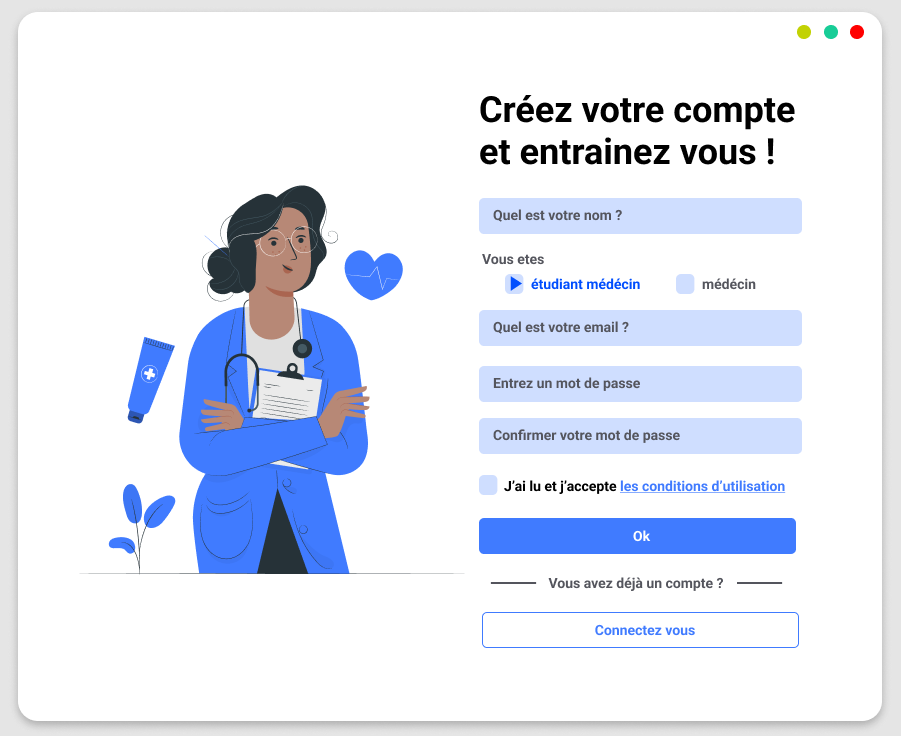
\includegraphics[width=\textwidth]{figures/signup.png}
    \captionsetup{justification=centering}
    \caption{Interface pour la création de compte}
    \label{fig:in_compte}
\end{figure}

\subsubsection{Interface de connexion}
Nous présentons à la figure \ref{fig:in_connection}  , l'interface qui sera vue par l'utilisateur lors de la réalisation du cas d'utilisation "Se Connecter".
\begin{figure}[H]
    \centering
    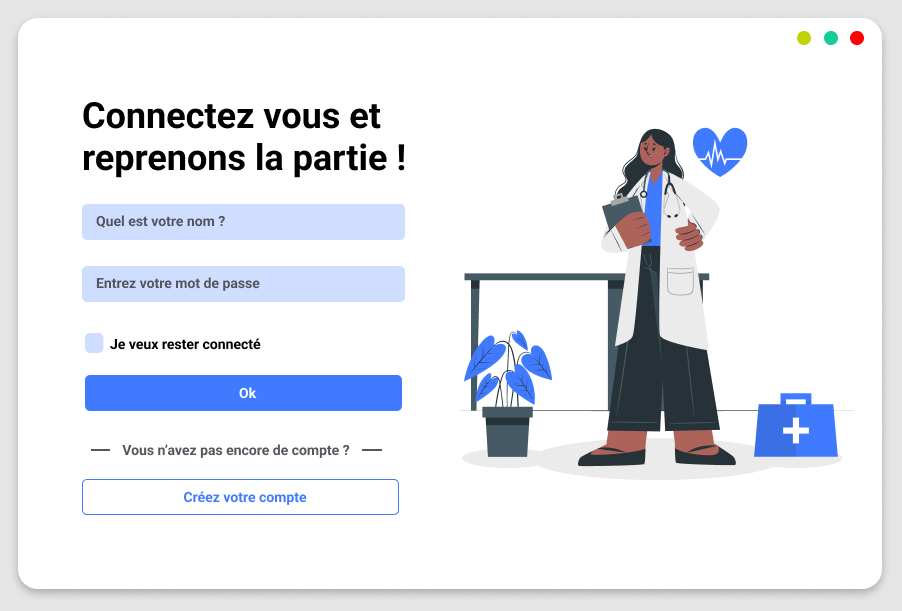
\includegraphics[width=\textwidth]{figures/signin.png}
    \captionsetup{justification=centering}
    \caption{Interface de Connexion}
    \label{fig:in_connection}
\end{figure}

\subsubsection{Interface du tableau de bord à la première connexion de l'utilisateur}
À la première connexion de l'utilisateur, un pré-test lui sera proposé afin de jauger son niveau pour la configuration de son premier exercice de diagnostic. À la figure \ref{fig:dashboard_first}, nous présentons l'interface qui sera vu par l'utilisateur.
\begin{figure}[H]
    \centering
    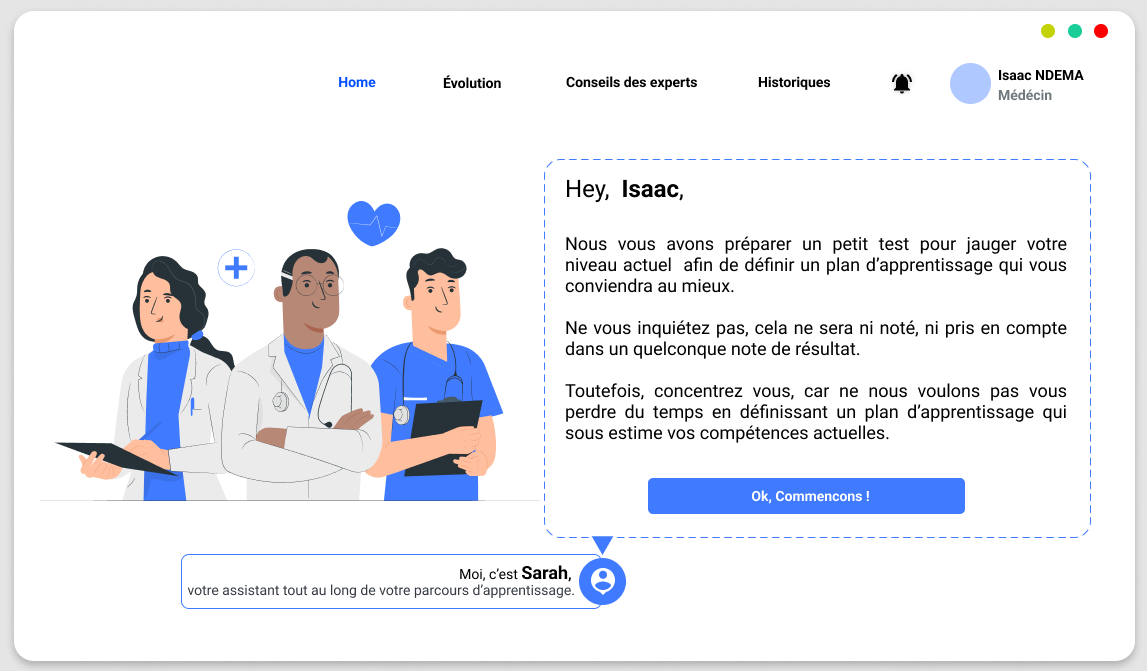
\includegraphics[width=\textwidth]{figures/dashboard-first-connection.png}
        \captionsetup{justification=centering}
    \caption{Interface du tableau de bord à la 1ère connexion}
    \label{fig:dashboard_first}
\end{figure}

\subsubsection{Interface du tableau de bord  de l'utilisateur}
Nous présentons à la figure \ref{fig:dashboard} , l'interface qui sera vue par l'utilisateur lors de la réalisation du cas d'utilisation "Lancer un exercice de diagnostic".
\begin{figure}[H]
    \centering
    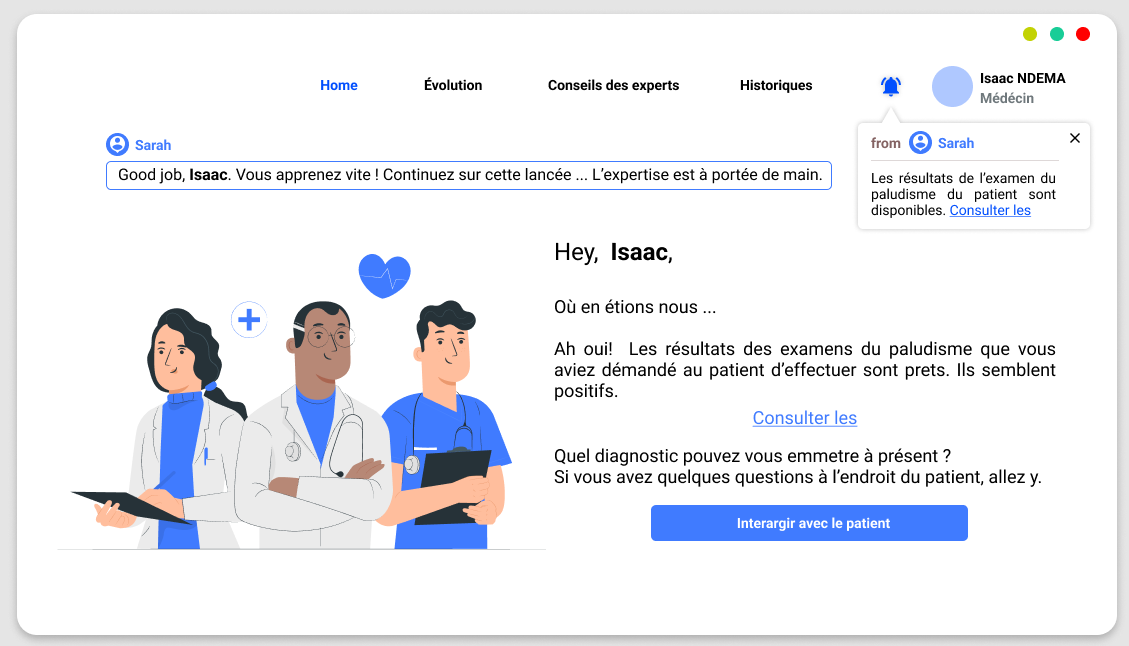
\includegraphics[width=\textwidth]{figures/dashboard.png}
        \captionsetup{justification=centering}
    \caption{Interface du tableau de bord}
    \label{fig:dashboard}
\end{figure}

\subsubsection{Interface de l'échange entre l'apprenant et le patient virtuel}
Nous présentons à la figure \ref{fig:echange} , l'interface qui sera vue par l'utilisateur lors d'un échange avec le patient virtuel.
\begin{figure}[H]
    \centering
    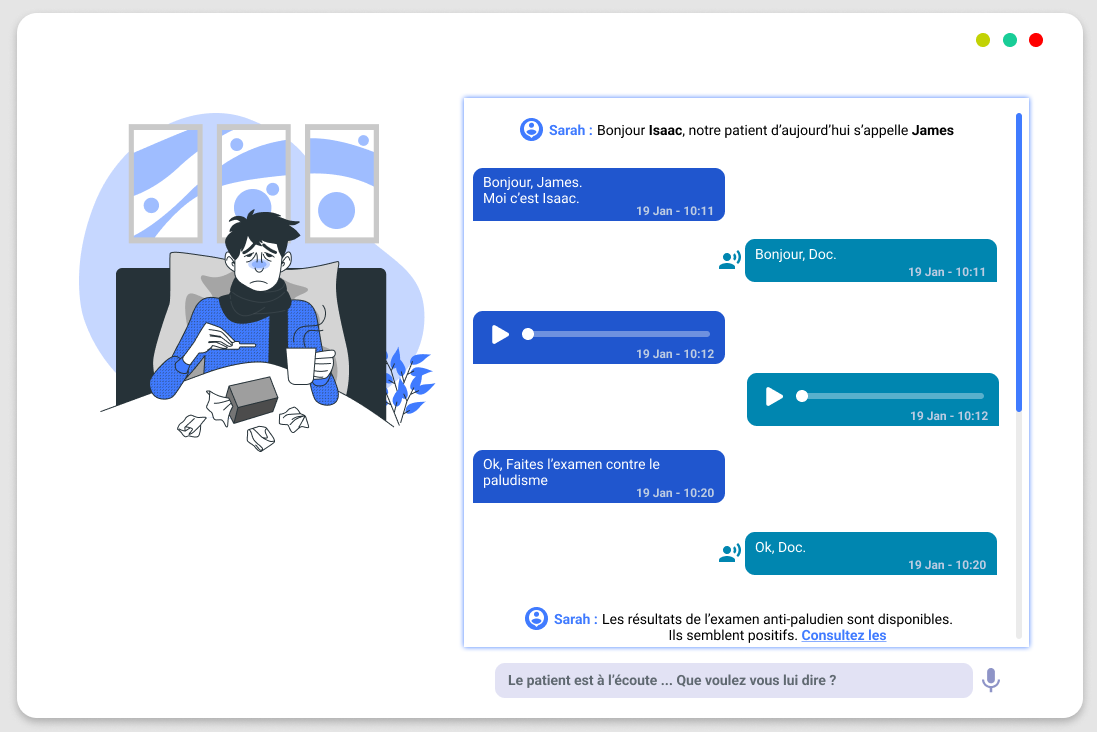
\includegraphics[width=\textwidth]{figures/patient-apprenant.png}
        \captionsetup{justification=centering}
    \caption{Interface de l'échange entre l'apprenant et le patient virtuel}
    \label{fig:echange}
\end{figure}

\section{Modèle apprenant}

\subsection{Modèle cognitif}

 En nous basant sur la littérature, nous avions le choix entre plusieurs méthodes de modélisation de l'apprenant dans un STI : réseaux sémantiques, banque de connaissances de l'expert , réseaux bayésiens, etc. Nous Nus sommes orientés vers le choix d'un réseau bayésien pour modéliser les connaissances et les compétences de l'apprenant même si l'une des grandes difficultés attendues sera l'absence de banque de données que nous pouvions exploiter pour construire la structure du réseau.\\\
\textbf{SARAH} est un système qui doit être capable d'adapter le processus d'apprentissage à chaque apprenant. Rendre possible cette adaptabilité requiert un modèle du domaine d'une part, et un modèle apprenant pour chaque joueur d'autre part, afin d 'offrir un soutien personnalisé (Le et Pinkwart, 2015). L'un des problèmes que l'on rencontre lors de la modélisation de l'apprenant est l'incertitude dans les croyances que le système a des connaissances de l'apprenant, et les sources d'incertitude sont nombreuses. En effet un apprenant peut commettre une erreur au courant du processus de résolution d 'un problème pourtant il possède les connaissances et les compétences pour réussir, ou encore parvenir à construire un schéma valide de résolution de manière tout à fait hasardeuse (D Baker et al., 2008) . Notre choix d 'utiliser \textbf{les réseaux bayésiens} pour modéliser l'apprenant devient alors judicieux, puisqu'ils offrent des mécanismes permettant de gérer l'incertitude (Woolf, 2010). 

Un réseau bayésien est un graphe orienté dans lequel chaque nœud est annoté avec des informations quantitatives de probabilité, et dont la spécification est la suivante (Russell et Norvig, 2010) :
\begin{enumerate}
\item Chaque nœud correspond à une variable aléatoire qui peut être discrète ou continue.
\item  Les paires de nœuds sont connectées par un ensemble de liens orientés. Un nœud X est dit parent d'un nœud Y s'il existe un lien orienté partant du nœud X vers le nœud Y. Le graphe décrit par le réseau bayésien est direct et acyclique (ne contient pas de cycles orientés).
\item  Chaque nœud Xi possède une distribution de probabilités P(Xi|Parents( Xi)) qui quantifie l'effet des parents sur le nœud. Pour les variables discrètes, cette distribution de probabilités est représentée par une table. 
\end{enumerate}
 

La construction d 'un réseau bayésien se fait généralement en trois étapes (Le et Pinkwart, 2015) : 
\begin{enumerate}
\item  Définir la structure du réseau bayésien (sa topologie). 
\item  Initialiser des valeurs des nœuds du réseau avec une estimation des connaissances et des compétences de l'apprenant. Cette étape influence grandement la manière dont le réseau est mis à jour pour refléter la progression de ce dernier.
\item Mettre à jour les probabilités dans le réseau bayésien en utilisant les informations tirées des interactions entre l'apprenant et le système.
\end{enumerate}
La mise en œuvre de ces trois étapes peut se faire suivant trois méthodes : 

\begin{itemize}
\item \textbf{A partir des connaissances du domaine ou des données existantes sur le domaine}. La tâche consiste à correctement identifier les objectifs de la modélisation (prédiction, explication ou exploration), identifier toutes les observations pertinentes pour le problème, déterminer lesquelles de ses observations seront représentées dans le modèle, définir à partir de ces observations, des variables ayant des états finis et mutuellement exclusifs, puis déterminer la distribution de probabilité pertinente pour le modèle (Heckerman, 2008).
\item \textbf{En sollicitant la collaboration des experts du domaine}. Il s'agit de se fier aux experts du domaine pour accomplir les tâches listées au point précédent. Seulement, s'appuyer sur le jugement d'experts est coûteux et peut être uj et à l'erreur, car il est difficile pour un humain de se fier à son intuition pour définir des dépendances probabilités réalistes entre des concepts. ( Conati, 2010) 
\item \textbf{Une combinaison des deux premières méthodes}.
\end{itemize}

 La modélisation de l'apprenant à l'aide d 'un réseau bayésien consiste donc en un ensemble de nœuds représentant les variables associées au processus d'apprentissage (connaissance, compétence, évidence, etc.), et d 'arcs représentant les relations entre ces nœuds qui peuvent être de deux types (Le et Pinkwart, 2015) : 
\begin{enumerate}
\item Relation entre une compétence et une unité de connaissance;
\item Relation entre une unité de connaissance et un nœud d'évidence. Les nœuds d'évidence sont ceux qu'on appelle des événements d'apprentissage et représentent les nœuds observables du réseau. Dans  \textbf{SARAH} par exemple, les nœuds observables caractérisent les actions que l'apprenant peut effectuer dans l'environnement durant un exercice. La figure 4.6 (Le et Pinkwart , 2015)  donne un exemple de réseau bayésien illustrant les deux types de relations énoncés dans le paragraphe précédent.\\\
\end{enumerate}

\begin{figure}[H]
    \centering
    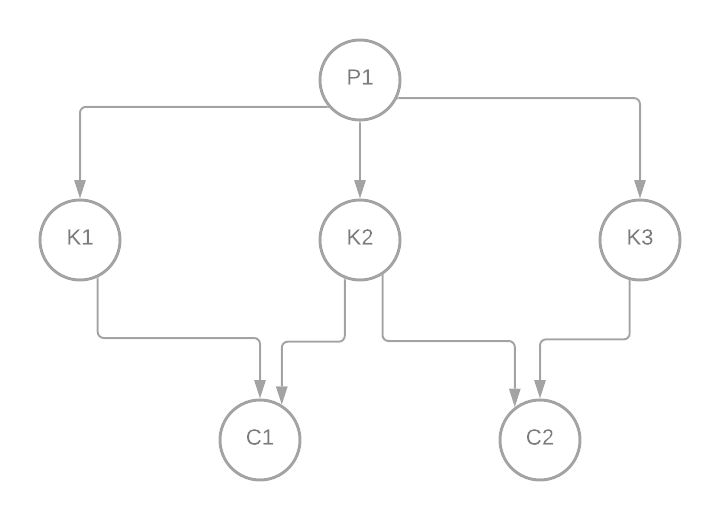
\includegraphics[width=\textwidth]{figures/r_by.png}
        \captionsetup{justification=centering}
    \caption{Exemple de réseau bayésien}
    \label{fig:r_by}
\end{figure}

Les relations de causalité entre les nœuds du réseau bayésien ci-dessus peuvent être interprétées comme suit : Si le problème Pl est résolu, l'apprenant a probablement acquis les connaissances Kl, K2 et K3. Si les connaissances Kl et K2 ont été acquises, l'apprenant possède probablement la compétence Cl. Si les connaissances K2 et K3 ont été acquises, l'apprenant possède probablement la compétence C2. 

Considérons les nœuds suivant d'un réseau bayésien : un problème P, une connaissance et une compétence C. La relation entre deux nœuds quelconques du réseau peut être exploitée dans les deux sens (Brusilovsky et Millan 2007) : 
\begin{itemize}
\item Le sens causal, (K→ P) ou (K → C); 
\item Le sens du diagnostic, ( P → K) ou ( C → K). 
\end{itemize}

Ce qui conduit à l'interprétation suivante dans le cas de modélisation de la relation entre une compétence et une connaissance (Le et Pinkwart, 2015) 
\begin{itemize}
\item  (K → C) : posséder la connaissance K indique la possibilité de posséder la compétence C;
\item ( C → K ) : posséder la compétence C signifie posséder la connaissance associée J-(. Ici, le nœud K peut être utilisé pour évaluer l 'approche de résolution de l'apprenant.  
\end{itemize}
